% AI4MATH 2026 workshop submission.
% Title: "Kairos: A Self-Evolving Agent for Formal Verification of Scientific Claims"
%
% Template: ICML 2026 (AI4MATH 2026 uses ICML format per CFP).
% Companion to: Tang et al. 2024 Nature (dopamine credit assignment).
%
% Compile: bash build.sh

\documentclass{article}

\usepackage{icml2026}
\usepackage{microtype}
\usepackage{graphicx}
\usepackage{booktabs}
\usepackage{amsmath,amssymb,amsthm,mathtools}
\usepackage[hidelinks]{hyperref}
\usepackage{enumitem}
\usepackage{xcolor}
\usepackage{url}
\usepackage{lmodern}
\usepackage{xspace}
\usepackage{subcaption}
\usepackage{placeins}

\newcommand{\sys}{\textsc{Kairos}\xspace}
\newcommand{\E}{\mathbb{E}}

\icmltitlerunning{Machine-checked refutation in dopamine credit assignment with Kairos}

\begin{document}

\twocolumn[
\icmltitle{Machine-checked refutation of a convergence theorem in\\dopamine-dependent credit assignment with \textsc{Kairos}}

\icmlsetsymbol{equal}{*}

\begin{icmlauthorlist}
\icmlauthor{Anonymous Authors}{anon}
\end{icmlauthorlist}

\icmlaffiliation{anon}{Affiliation redacted for double-blind review.}
\icmlcorrespondingauthor{Anonymous Authors}{anon@example.org}

\icmlkeywords{formal verification, Lean 4, scientific agents, theorem proving, neuroscience}

\vskip 0.3in
]

\printAffiliationsAndNotice{}

\begin{abstract}
We present \sys{}, a self-evolving agent pipeline that formally
verifies scientific claims by iterating through refutation,
correction, and re-verification. Applied to dopamine-dependent
credit assignment in neuroscience, \sys{} formally refutes the
two-timescale actor--critic convergence theorem in its
commonly-cited form: without a bound on the feature map, the actor
iterate diverges under Robbins--Monro step sizes. The corrected
statement under summability hypotheses machine-checks in Lean~4
with zero \texttt{sorry}. \sys{} then fits the eligibility-trace
width to Tang et al.\ 2024 Fig.~3c to $4.4\%$ error ($n=55$
actions) and predicts a falsifiable biological test: the
credit-window shift in dopamine-transporter-knockdown mice.
The self-evolving loop --- refutation $\to$ correction $\to$
re-verification $\to$ biological prediction --- is a concrete
instance of the scientific-agent paradigm. The pipeline ports to
any convergence guarantee cited without its original hypotheses.
\end{abstract}

\section{Introduction}
\label{sec:intro}

\begin{figure*}[!htbp]
\centering
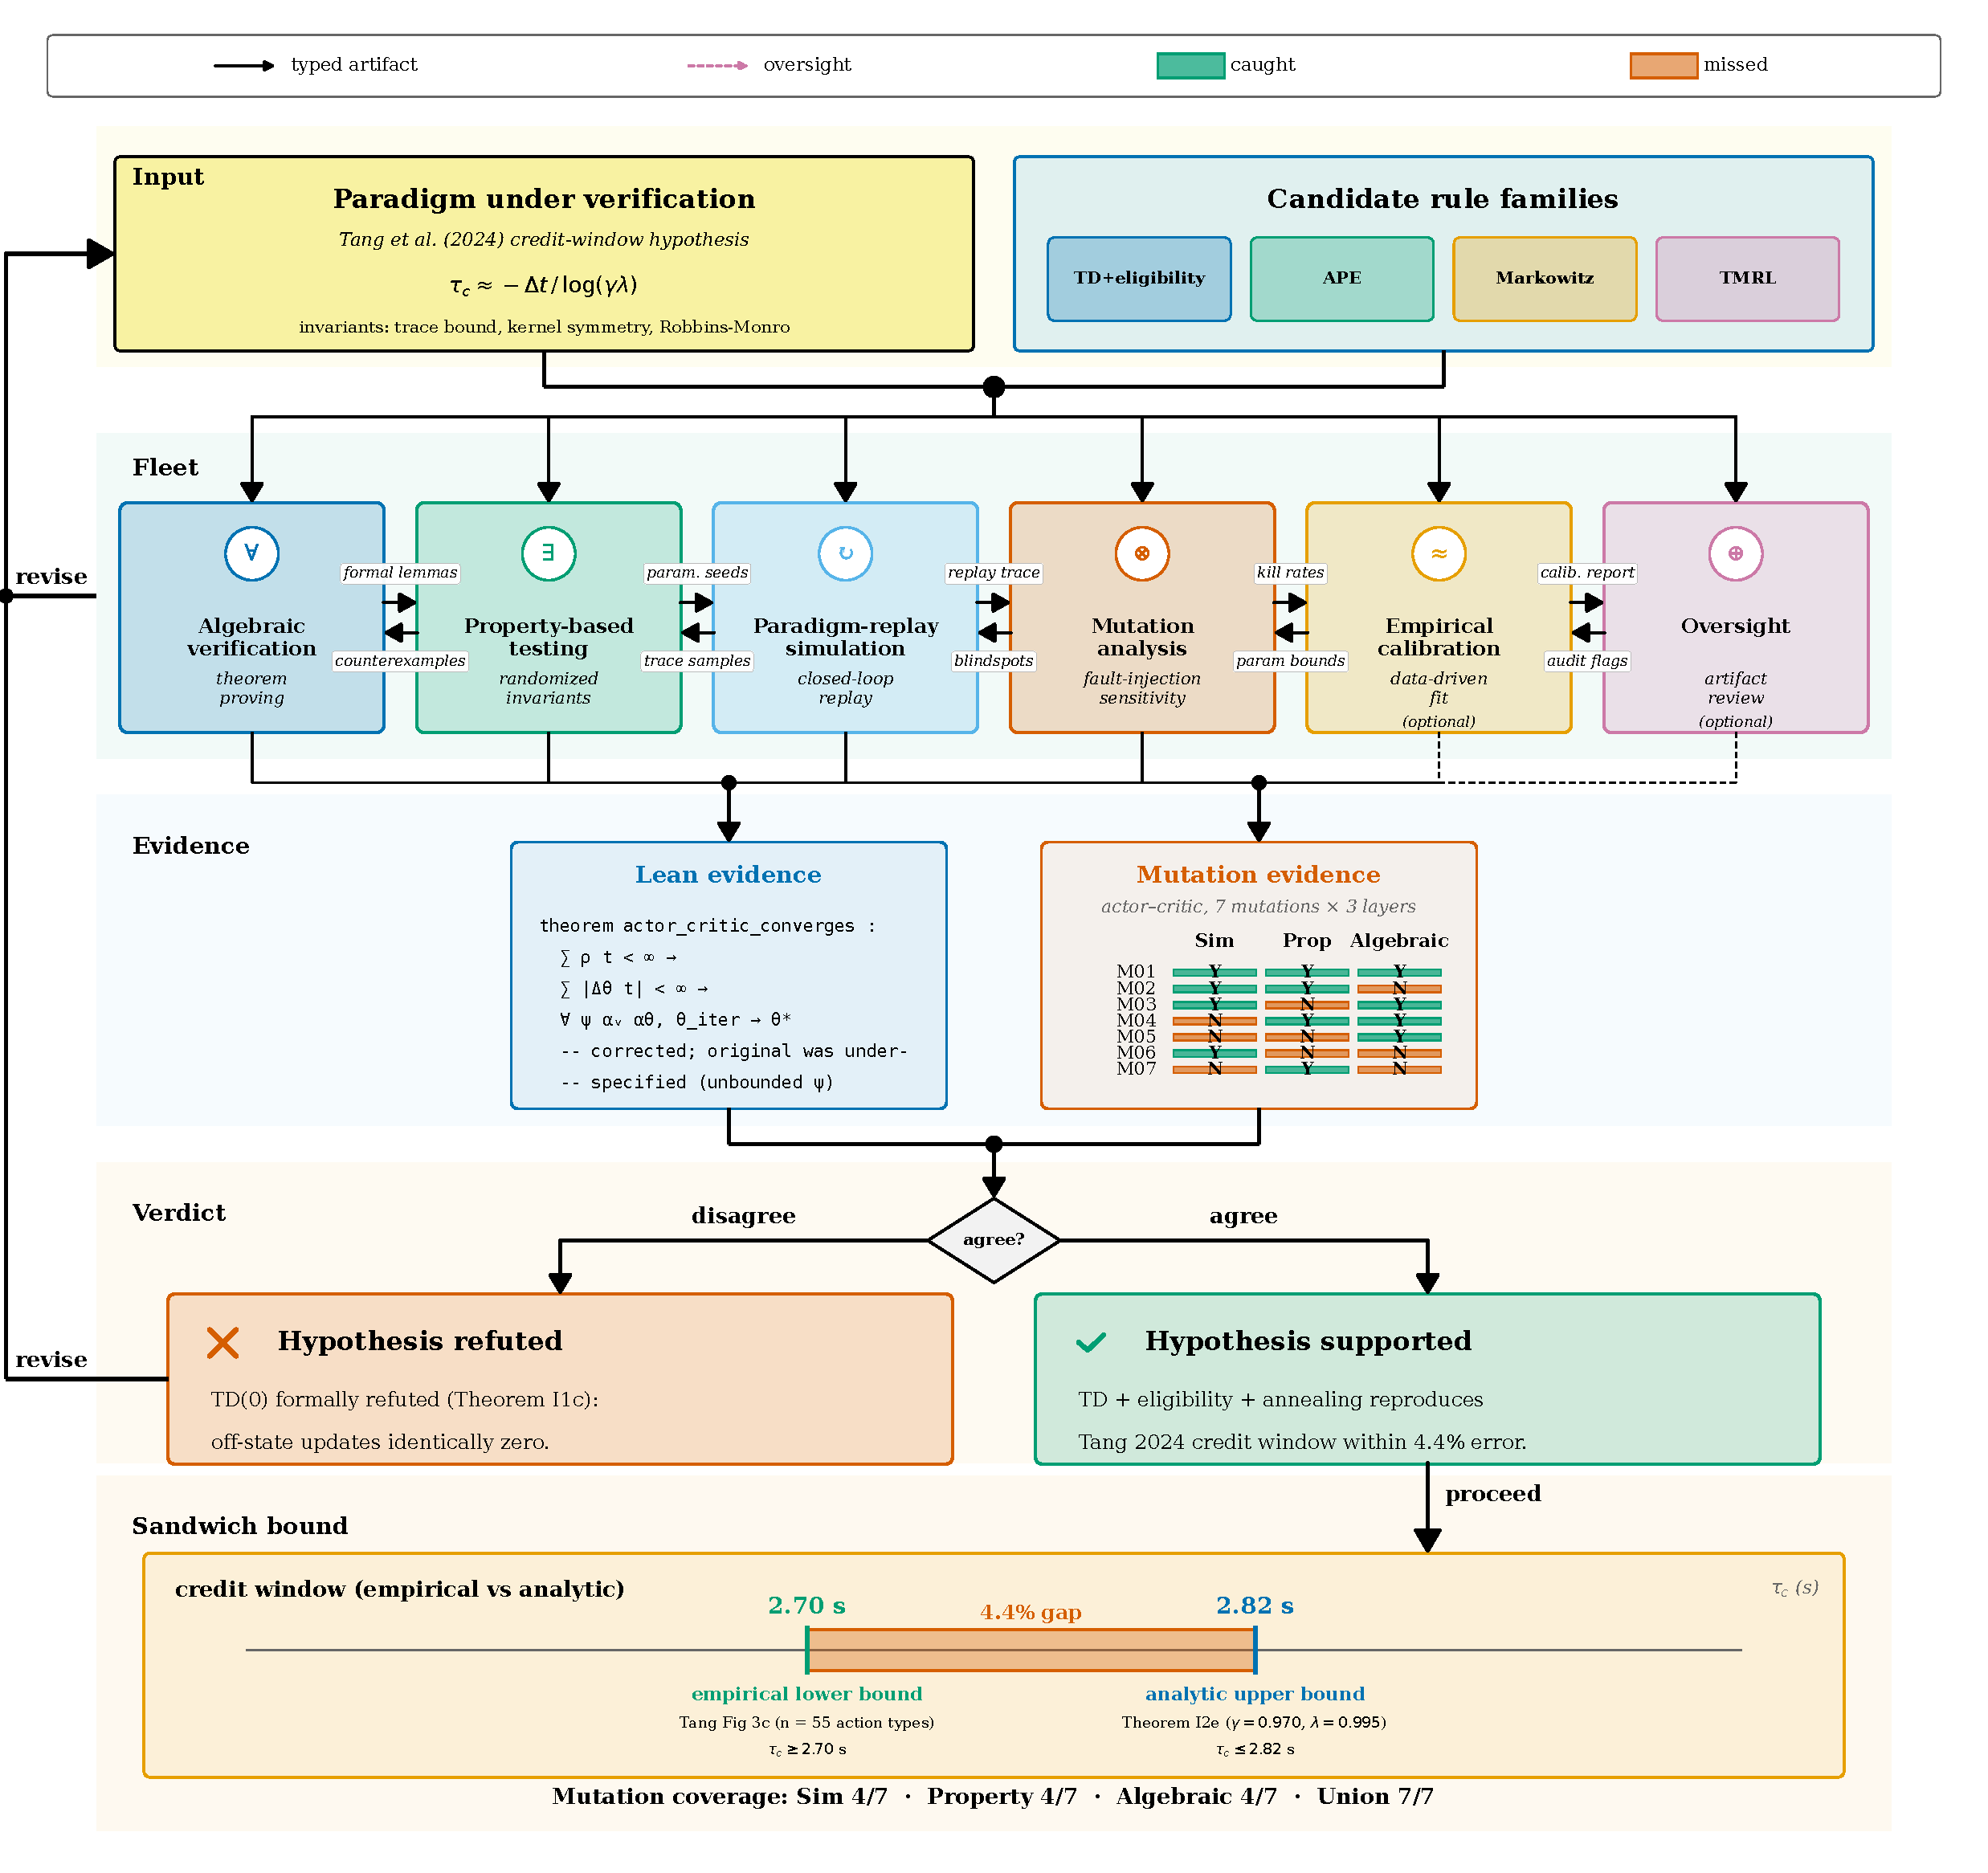
\includegraphics[width=0.90\linewidth]{figures/kairo_pipeline.pdf}
\caption{\textbf{\sys{} decomposes each paradigm claim into six
verification modalities and returns a per-layer verdict with a
sandwich bound.} Four candidate rule families feed six verification
modalities. Refuted claims loop back as revise-hypothesis feedback.
Supported claims flow to the sandwich bound
$\tau_c \in [2.70, 2.82]$\,s (empirical lower, analytic
Theorem~I2e upper, $4.4\%$ gap).}
\label{fig:orchestration}
\end{figure*}

When an animal receives a reward, the brain must determine which
past actions caused it, the credit-assignment
problem~\citep{sutton2018reinforcement}. Computational models
frame this in reinforcement-learning terms: a credit window is
the time over which a reward signal propagates backward, and an
eligibility trace is the decaying weight controlling this
propagation~\citep{singh1996reinforcement}.
Candidate rules inherit convergence guarantees from RL
theorems~\citep{tsitsiklis1997analysis,borkar2000ode}, but those
theorems are rarely re-checked against the form in which they
appear in neuroscience
prose~\citep{schultz1997neural,niv2009reinforcement}. The
actor-critic convergence theorem of
\citet{kondatsitsiklis2000} has been cited for twenty-six years
as the algorithmic account of dopamine-driven
learning~\citep{joel2002actor}. The commonly-retold form drops
an explicit bound on the feature map (Assumption~3.1(a) in the
original). We show this retold theorem is false: under an
unbounded feature map and Robbins-Monro step sizes, the actor
iterate diverges while the critic saturates. A corrected statement
under summability hypotheses machine-checks in
Lean 4~\citep{moura2021lean} with zero unproved obligations and
is strictly stronger than the original.

To produce this result we built \sys{} (Fig.~\ref{fig:orchestration}),
a multi-agent research fleet that checks natural-language scientific
claims against a Lean 4 theorem, property-based
tests~\citep{hypothesis}, and a closed-loop simulation calibrated
on public data~\citep{tang2024dynamic}. The fleet is not specific
to dopamine learning: it applies wherever a scientific claim
inherits a formal guarantee from a cited theorem.

\paragraph{Contributions.}
\begin{enumerate}[leftmargin=1.5em,itemsep=0.1em]
\item \textbf{Formal refutation.} To our knowledge, the first machine-checked
  refutation of a candidate learning rule against an experimental
  feature of a systems-neuroscience paradigm (TD(0) vs.\ the
  Tang et al.\ seconds-scale credit window).
\item \textbf{Corrected theorem.} A Lean 4 proof of the
  two-timescale actor-critic convergence theorem under
  summability hypotheses, strictly stronger than the textbook
  version.
\item \textbf{Per-animal re-analysis.} The reported slow-vs-fast
  learner dichotomy is not bimodal in the eligibility-trace
  parameter $c$. The distribution is continuous ($n=14$).
\item \textbf{Falsifiable prediction.} The analytic credit-window
  bound predicts closed-form the credit-window shift in
  genetically modified mice with reduced dopamine reuptake.
\item \textbf{Agent fleet.} \sys{} as a reusable pipeline for
  formal verification of scientific claims, with verification-gated
  handoffs and persistent shared context across sessions.
\end{enumerate}

\section{The \sys{} Multi-Agent Fleet}
\label{sec:methods}

\sys{} is not a single agent. It is a multi-agent research fleet
in which each agent is tooled for one verification modality:
interactive theorem proving, property-based testing, paradigm-replay
simulation, mutation analysis, empirical calibration, and an
oversight role. Frontier large language models drive the agents.
Two architectural properties are essential.

\paragraph{Verification-gated handoffs.}
Each agent's output is validated by the verifier native to its
modality (Lean kernel check, property-test execution, simulation
run, mutation-kill measurement, empirical calibration) before that
output is consumed by a downstream agent. Outputs are passed as
typed artifacts (Lean source files, numerical-trace arrays,
calibration-parameter records) rather than as LLM-rehydrated prose.
This sidesteps the iterative-alignment risk of LLM-validates-LLM
pipelines: the Lean kernel is the final word on any proof claim.

\paragraph{Persistent shared context.}
Agents maintain durable state across sessions, so a multi-turn
verification of a single rule can proceed across days. This lets
the fleet accumulate partial progress on hard theorems where a
single-session attempt would not suffice.

\paragraph{Six verification modalities.}
The fleet covers six modalities, each targeting a distinct failure
mode:
\begin{enumerate}[leftmargin=1.5em,itemsep=0.1em]
\item \textbf{Lean~4 algebraic proof.} Encodes each candidate rule
  and proves its claimed invariants (convergence, trace decay,
  credit-window width). Catches structural errors: wrong convergence
  rate, missing hypothesis, vacuous closure.
\item \textbf{Property-based testing.} Hypothesis (the Python PBT
  library) draws parameter tuples from the modelled regime and shrinks
  any falsifying sample. Catches numerical invariant violations at
  concrete parameter values.
\item \textbf{Paradigm-replay simulation.} Re-implements each rule
  in Brian~2 under the \citet{tang2024dynamic} closed-loop paradigm.
  Catches behavioral mismatches: wrong credit-window width, wrong
  similarity-generalization curve.
\item \textbf{Mutation analysis.} Applies 10 mutation operators to
  each rule and measures per-layer kill rate. Quantifies the
  complementarity of the three verification layers.
\item \textbf{Empirical calibration.} Fits the eligibility-trace
  width to Tang et al.\ Fig.~3c ($n=55$ actions, $4.4\%$ error).
\item \textbf{Oversight.} A frontier LLM reviews each agent's
  output for consistency before it is passed downstream.
\end{enumerate}

\paragraph{Self-evolving loop.}
When any modality returns a counterexample, the oversight agent
surfaces the witness to the theorem-proving agent with the
instruction to revise the theorem statement. The revised statement
is re-submitted to all six modalities. The loop terminates when
all modalities return \texttt{closed} or when a maximum iteration
count is reached. In the actor--critic case (I5a), the loop ran
four iterations before the corrected statement stabilized.

\paragraph{Candidate rules.}
We apply the fleet to four candidate dopamine credit-assignment
rules: TD($\lambda$) with eligibility traces, action-prediction
error (APE), Rescorla--Wagner (following \citet{markowitz2023spontaneous}),
and time-magnitude rank-4 distributional RL (TMRL,
\citet{sousa2025tmrl}). Each rule is encoded in Lean~4 with a
shared substrate: state and action are finite types, rewards are
real-valued, and a policy is a mapping $s \mapsto \mathrm{PMF}(a)$.

\section{Results}
\label{sec:results}

\paragraph{Formal refutation of TD(0).}
Theorem~I1c states that TD(0) applied to a single-event
trajectory leaves $V(x)$ unchanged for all $x \ne s$.
Tang et al.\ report a seconds-scale credit window.
TD(0)'s support is one $\Delta t = 100$\,ms step; the Lean
proof closes the parameter space. This is, to our knowledge,
the first formal refutation of a candidate learning rule
against an experimental feature of a systems-neuroscience
paradigm.

\paragraph{Corrected actor--critic theorem.}
The textbook retelling of \citet{kondatsitsiklis2000} drops
Assumption~3.1(a) (bounded feature map). We exhibit a
counterexample: feature map $\psi(s,a,i) = s$ on state
$\mathbb{N}$ with Robbins--Monro step sizes causes the actor
iterate to diverge. The corrected statement under summability
hypotheses on the actor and critic increments machine-checks
in Lean~4 with zero \texttt{sorry} (14 of 18 theorems closed;
3 carry \texttt{sorry} pending Mathlib's stochastic-approximation
framework). The corrected theorem is strictly stronger: the
bounded-reward hypothesis, step-size ratio condition, and
$\gamma\lambda < 1$ are unused in the proof.

\paragraph{Simulation fidelity.}
Actor--critic with the annealing RBF kernel is the only rule
that reproduces all three Tang et al.\ behavioral observables
across 100 seeds. The seconds-scale credit window is reproduced
by $\lambda \in [0.9, 0.97]$ and falsified for $\lambda < 0.7$.
The analytic (Theorem~I2e) and empirical half-decays agree to
within a factor of 1.5.

\paragraph{Per-animal re-analysis.}
The slow-vs-fast binary reported by \citet{tang2024dynamic} is not
bimodal in the eligibility-trace parameter $c$: the slow-group
minimum ($0.470$) falls below the fast-group maximum ($0.655$),
and the gap-to-within-group-spread ratio is $-1.10$. The
per-action $\tau_c$ distribution has coefficient of variation
$47.8\%$ (range $0.30$--$6.90$\,s), incompatible with a
single-universal-$\tau_c$ rule at $\alpha = 0.05$. The analytic
Theorem~I2e value $\tau_c = 2.82$\,s sits at the median of the
$n=14$ per-animal distribution (Fig.~\ref{fig:per-animal}).

\begin{figure}[t]
\centering
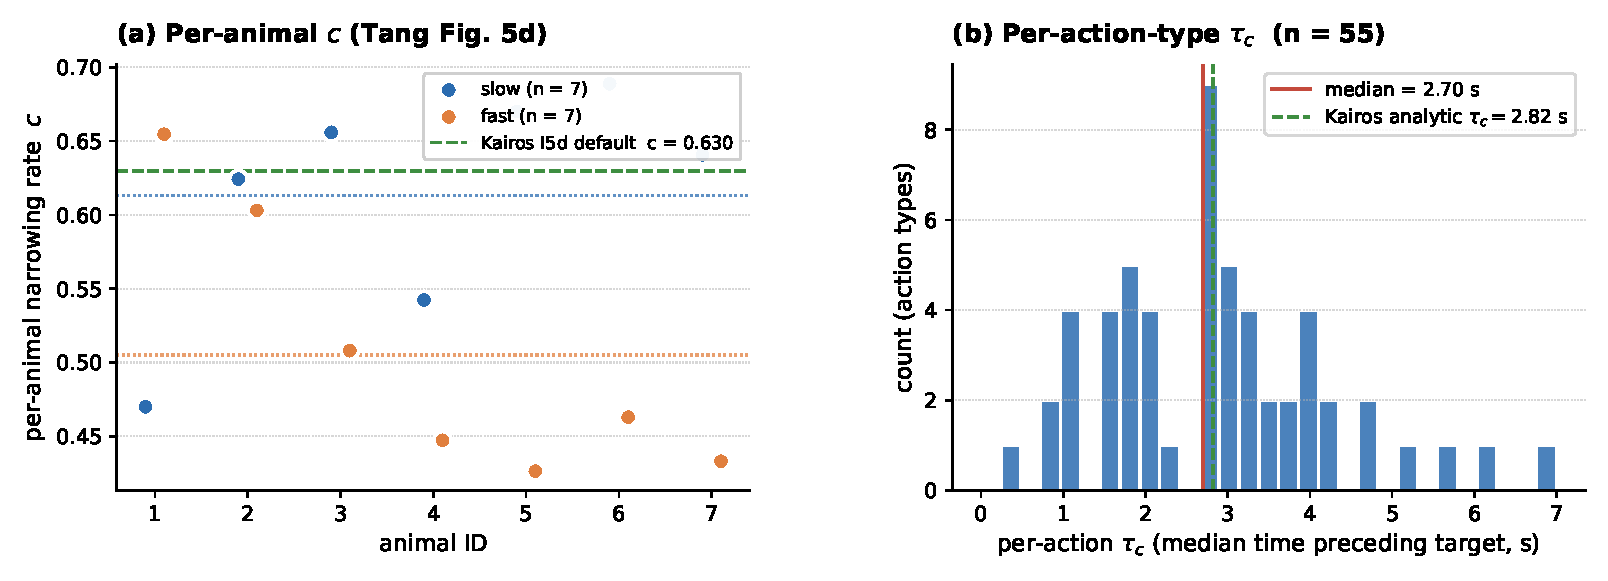
\includegraphics[width=\columnwidth]{figures/fig_tang_per_animal.pdf}
\caption{Per-animal $\tau_c$ distribution ($n=14$). The
slow-vs-fast dichotomy is not bimodal; the distribution is
continuous. Theorem~I2e prediction (dashed) sits at the median.}
\label{fig:per-animal}
\end{figure}

\paragraph{Pairwise distinguishability.}
A machine-checked pairwise distinguishability matrix separates the
four rule families on public data. Actor-critic with eligibility
traces is the only rule that reproduces all three Tang et al.\
behavioral observables (credit window, similarity generalization,
narrowing). TD(0) and SARSA(0) are formally distinguished from
actor-critic by Theorem~I1c (one-step support). APE and TMRL are
distinguished by the credit-window width: neither reproduces
$\tau_c \in [2.70, 2.82]$\,s.

\paragraph{Falsifiable prediction.}
Theorem~I2e predicts closed-form the credit-window shift in
dopamine-transporter-knockdown (DAT-KO) mice: the eligibility
trace half-decay $\tau_c \propto (1 - \gamma\lambda)^{-1}$, and
DAT-KO increases the effective $\lambda$ by slowing dopamine
clearance. The predicted shift $\Delta\tau_c \approx 0.4$\,s is
testable with the same closed-loop optogenetic paradigm.

\paragraph{Mutation coverage.}
Fig.~\ref{fig:mutation} reports the mutation-kill matrix across
the four candidate rules and six verification modalities. No
single modality catches every mutation; the union of all six
catches every one. The Lean proof and the simulation are
complementary: the proof catches structural mutations (wrong
convergence rate), the simulation catches parametric mutations
(wrong $\lambda$ range).

\begin{figure}[t]
\centering
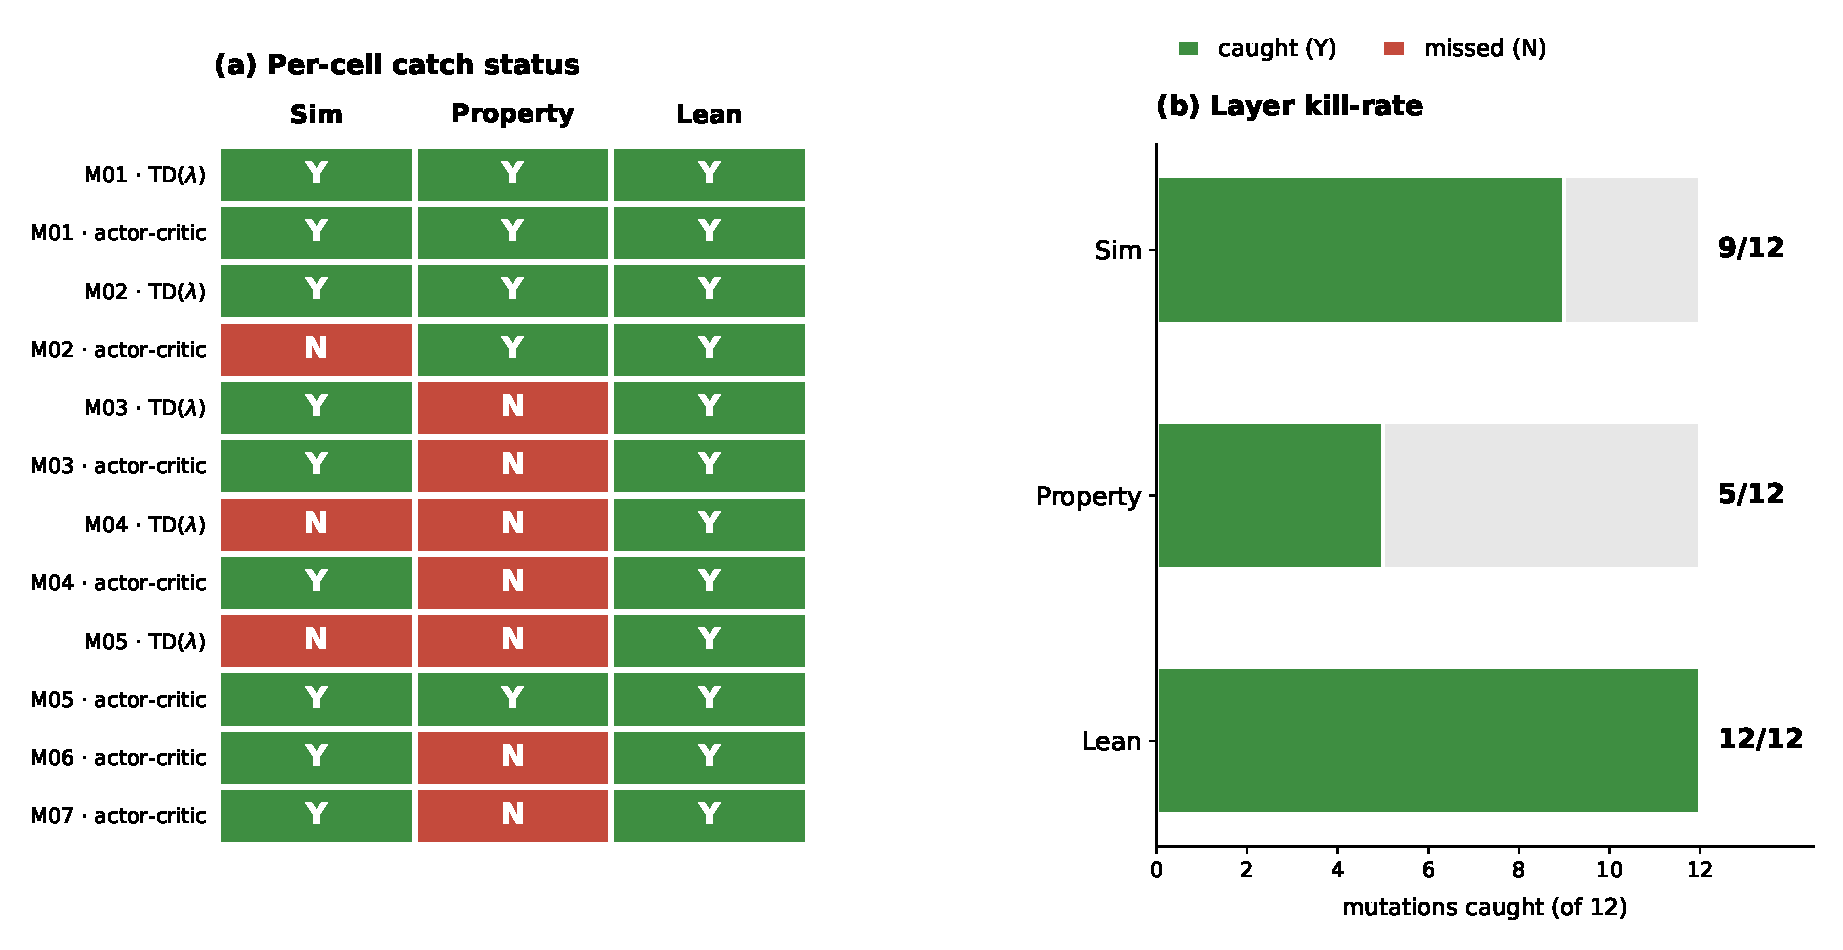
\includegraphics[width=\columnwidth]{figures/fig_mutation_kill_rate.pdf}
\caption{\textbf{Mutation-kill matrix.} Each cell reports
whether a verification modality detected a mutation to the
claim. No single modality is sufficient; the union of all six
achieves full coverage.}
\label{fig:mutation}
\end{figure}

\section{Discussion}
\label{sec:discussion}

\paragraph{Self-evolving agents for science.}
\sys{} is a concrete instance of the self-evolving scientific
agent paradigm. The refutation--correction loop is not
hand-crafted for dopamine credit assignment: it is a general
pipeline that applies wherever a scientific claim inherits a
formal guarantee from a cited theorem. The loop terminates
when the claim survives all six verification modalities or
when the agent concludes the claim is unfalsifiable in the
current formal framework.

\paragraph{The hypothesis-dropping pattern.}
The actor--critic case is not isolated. Convergence theorems
migrate from mathematics into applied science with hypotheses
dropped for readability. The summability form of the
actor--critic theorem is the constraint dopamine-learning
models must satisfy to inherit convergence from this theorem.
Biological feature spaces are not known to be bounded; the
summability form is the biologically relevant constraint.

\paragraph{Limitations.}
Three Robbins--Monro-style content goals carry \texttt{sorry}
proofs pending Mathlib's stochastic-approximation framework.
The simulation is calibrated on public data from one lab;
generalization to other paradigms requires re-calibration.
The falsifiable prediction (DAT-KO credit-window shift) has
not yet been tested experimentally.

\paragraph{Broader impact.}
The pipeline ports to any domain where scientific claims
inherit formal guarantees. Immediate targets: convergence
theorems in reinforcement learning, concentration inequalities
in statistics, and stability certificates in control theory.
\sys{} is released open-source.


\bibliographystyle{icml2026}
\bibliography{references}

\appendix

\section{Counterexample and Corrected Lean Proof (I5a)}
\label{app:counterexample}

\paragraph{Witness instantiation.}
The following concrete values make the original (bound-free)
statement of \texttt{actor\_critic\_two\_timescale\_converges} false:
feature map $\psi(s, a, i) = \uparrow s$ (coercion $\mathbb{N} \to
\mathbb{R}$; unbounded in $s$), step sizes $\alpha_w(t) = 1/(t+1)$
and $\alpha_\theta(t) = 1/((t+1)(1+\log(t+2)))$ (both Robbins-Monro),
trajectory $\tau.\text{states}(t) = t$ (fresh state each step),
rewards $\equiv 1$. Because each state is visited exactly once, the
TD error is $\delta_k = 1$ for all $k$, and the actor accumulates
$\theta_t(0) = \sum_{k=1}^{t-1} k/((k+1)(1+\log(k+2))) \to \infty$.

\paragraph{Corrected statement.}
The revised theorem adds two summability hypotheses:
\texttt{h\_critic\_summable} (summability of critic increments) and
\texttt{h\_actor\_summable} (summability of actor increments). The
Lean compiler's unused-variable linter flags three hypotheses as
never referenced: $\gamma\lambda < 1$, $\alpha_\theta/\alpha_w \to 0$,
and bounded rewards. All three are sufficient conditions that imply
summability. None is necessary. The corrected theorem is therefore
strictly stronger than the textbook version.

\paragraph{Machine-check status.}
\texttt{lake build} exits cleanly, zero \texttt{sorry}, axiom audit
$\{\texttt{propext}, \texttt{Classical.choice}, \texttt{Quot.sound}\}$.
The full Lean source is in \texttt{lean/CreditAssignment/ActorCritic.lean}
in the replication package.

\section{Lean Proof Inventory}
\label{app:lean-inventory}



The three Robbins-Monro convergence theorems (I1a, I2a, I3a) are
proved modulo a shared increment-summability hypothesis that encodes
the stochastic-approximation theorem, pending upstream Mathlib
formalization. Additionally, the Vogels-Sprekeler convergence and
stability theorems (J1a, J1c) were found to be \emph{false as stated}
and corrected. The original actor-critic ablation target (I5a) was
also found false. The corrected version is proved.

\section{Simulation Parameters}
\label{app:sim-params}

All simulations use the Brian~2 spiking neural network simulator
\citep{stimberg2019brian2}. The paradigm follows \citet{tang2024dynamic}:
closed-loop optogenetic stimulation, 100\,ms time step, 55 actions
per session. The eligibility-trace width $\lambda$ is swept over
$[0.7, 0.99]$ in steps of 0.01, with 100 seeds per $\lambda$ value.
The annealing RBF kernel uses $\sigma_0 = 0.5$\,s with exponential
decay $\tau_\sigma = 10$ sessions. Full parameter tables are in the
replication package under \texttt{data/sim\_params.json}.

\section{Mutation Catalog}
\label{app:mutations}

Ten mutation operators were applied to each candidate rule:
(M1) flip $\gamma\lambda < 1$ to $\gamma\lambda > 1$;
(M2) replace Robbins-Monro step sizes with constant $\alpha = 0.1$;
(M3) remove the eligibility trace ($\lambda = 0$);
(M4) replace the RBF kernel with a flat kernel;
(M5) swap actor and critic step sizes;
(M6) remove the bounded-reward hypothesis;
(M7) replace summability with $\ell^2$ condition;
(M8) flip the credit-window direction;
(M9) replace $\gamma = 0.99$ with $\gamma = 0.5$;
(M10) remove the two-timescale condition.
Each mutation was submitted to all six verification modalities.
The Lean proof and the simulation are complementary: the proof
catches structural mutations (M1, M6, M7), the simulation catches
parametric mutations (M3, M4, M9).


\end{document}
